\documentclass[12pt, letterpaper]{report}
\usepackage{enumitem}
\usepackage[a4paper, margin=0.7in, top=20mm, bottom=20mm]{geometry}
\usepackage{mathspec}
\usepackage[UTF8]{ctex}
\usepackage[colorlinks=true, linkcolor=black, urlcolor=blue]{hyperref}
\usepackage{listings}
\usepackage{xcolor}
\usepackage{graphicx}
\usepackage{xparse}
\usepackage{tcolorbox}
\usepackage{mdframed}

\graphicspath{ {./pics/} }

% ---- Code Section Style ----
\colorlet{mygray}{black!30}
\colorlet{mygreen}{green!60!blue}
\colorlet{mymauve}{red!60!blue}

\tcbuselibrary{breakable}
\NewDocumentCommand{\exercise}{ m +m }{
    {
        \edef\originalParIndent{\the\parindent}
        \begin{tcolorbox}[breakable,arc=0mm,boxrule=0.8pt]
            \setlength{\parindent}{\originalParIndent}
            \noindent
            \textbf{\large Exercise #1}
            \indent
            #2
        \end{tcolorbox}
    }
}

\tcbuselibrary{breakable}
\NewDocumentCommand{\question}{ m +m }{
    {
        \edef\originalParIndent{\the\parindent}
        \begin{tcolorbox}[breakable,arc=0mm,boxrule=0.8pt]
            \setlength{\parindent}{\originalParIndent}
            \noindent
            \textbf{\large Question}
            \indent
            #2
        \end{tcolorbox}
    }
}

\tcbuselibrary{breakable}
\NewDocumentCommand{\challenge}{ m +m }{
    {
        \edef\originalParIndent{\the\parindent}
        \begin{tcolorbox}[breakable,arc=0mm,boxrule=0.8pt]
            \setlength{\parindent}{\originalParIndent}
            \noindent
            \textbf{\large Challenge!}
            \indent
            #2
        \end{tcolorbox}
    }
}

\lstdefinelanguage
   [x64]{Assembler}     % add a "x64" dialect of Assembler
   [x86masm]{Assembler} % based on the "x86masm" dialect
   % with these extra keywords:
   {morekeywords={CDQE,CQO,CMPSQ,CMPXCHG16B,JRCXZ,LODSQ,MOVSXD, %
                  POPFQ,PUSHFQ,SCASQ,STOSQ,IRETQ,RDTSCP,SWAPGS, %
                  rax,rdx,rcx,rbx,rsi,rdi,rsp,rbp, %
                  r8,r8d,r8w,r8b,r9,r9d,r9w,r9b, %
                  r10,r10d,r10w,r10b,r11,r11d,r11w,r11b, %
                  r12,r12d,r12w,r12b,r13,r13d,r13w,r13b, %
                  r14,r14d,r14w,r14b,r15,r15d,r15w,r15b}} % etc.


\lstset{
  backgroundcolor=\color{gray!10},  
  basicstyle=\ttfamily,
  columns=fullflexible,
  breakatwhitespace=false,      
  breaklines=true,                
  captionpos=b,                    
  commentstyle=\color{mygreen}, 
  extendedchars=true,              
  frame=single,                   
  keepspaces=true,             
  keywordstyle=\color{blue},                    
  numbers=none,                
  numbersep=5pt,                   
  numberstyle=\tiny\color{blue}, 
  rulecolor=\color{mygray},        
  showspaces=false,               
  showtabs=false,                 
  stepnumber=5,                  
  stringstyle=\color{mymauve},    
  tabsize=3,                      
  title=\lstname                
}

\lstdefinestyle{CStyle}{  
    % commentstyle=\color{mGreen},
    % keywordstyle=\color{magenta},
    % numberstyle=\tiny\color{mGray},
    % stringstyle=\color{mPurple},
    basicstyle=\footnotesize,
    breakatwhitespace=false,                              
    showstringspaces=false,
    language=C
}

\lstdefinestyle{AssemblyStyle}{  
    basicstyle=\footnotesize,
    breakatwhitespace=false,                              
    showstringspaces=false,
    language=[x64] Assembler
}


\lstdefinestyle{MakeFileStyle}{  
    basicstyle=\footnotesize,
    breakatwhitespace=false,                              
    showstringspaces=false,
    language=[gnu] make
}


\setitemize[1]{itemsep=0pt,partopsep=0pt,parsep=\parskip,topsep=5pt}

% ----------------------------


\setcounter{chapter}{0}
\setlength{\parindent}{2em}
\setmainfont{Times New Roman}
\setcounter{tocdepth}{1}
\setcounter{secnumdepth}{1}

\title{MIT6.828 Lab3: User Environments}
\author{Zhuofan Zhang}
\date{Jan 2022}



\begin{document}
\maketitle
% ---- Contents ----
\pagenumbering{roman}
\renewcommand\contentsname{\Huge Contents}
\tableofcontents{}
% ------------------


% ---- Part A ---------------------------------
\newpage
\pagenumbering{arabic}
\chapter[\Large User Environments and Exception Handling]{User Environments and Exception Handling}
本次Lab的第一部分主要要处理JOS对进程的抽象及异常处理两部分的内容。

\section[\large Environment State]{Environment State}
JOS对进程(Process/Environment)的抽象位于 inc/env.h 及 kern/env.c中,包括结构体  
struct Env 及一系列接口。系统使用三个全局变量:envs, curenv, env\_free\_list 对所有用户进程及当前进程进行管理。\par
对于每一个用户进程,JOS使用 struct Env 表示:
\lstset{style=CStyle}
\setmainfont{Consolas}
\begin{lstlisting}
struct Env {
    struct Trapframe env_tf;	// Saved registers
    struct Env *env_link;		// Next free Env
    envid_t env_id;			// Unique environment identifier
    envid_t env_parent_id;		// env_id of this env's parent
    enum EnvType env_type;		// Indicates special system environments
    unsigned env_status;		// Status of the environment
    uint32_t env_runs;		// Number of times environment has run

    // Address space
    pde_t *env_pgdir;		// Kernel virtual address of page dir
};
\end{lstlisting}
\setmainfont{Times New Roman}
其中,当空闲 env 被放入 env\_free\_list 中时依靠 env\_link 构建链表。\par
JOS 的 Environment 组成与 *nix系统相似,由 {\bf Thread} 和 {\bf Address Space} 两部分概念组成:
前者由 env\_tf 中的寄存器描述(即进程切换时需保存的现场),后者由 env\_pgdir 指向的页表目录描述。\par
\textsl{注: JOS 与 xv6 设计存在差异。JOS 采用的是 Single Kernel Stack 的设计,一次只能有一个进程陷入内核;
而xv6的每个进程都拥有独立的内核栈(xv6的进程由 struct proc 描述)。}\par
\newpage
在上述 Env 结构体中,需要注意用于记录进程当前状态的 env\_status 变量。在 JOS 的设计中进程总共有5种可能
的状态:\par
\quad \par 

\begin{tabular}{|l|l|}
    \hline  
    \textbf{Status}&\textbf{Annotation}\\
    \hline 
    ENV\_FREE&表示进程尚未被分配,此时应处于 env\_free\_list 中\\
    \hline 
    ENV\_RUNNABLE&表示进程已被分配且可在下次进程切换时被调度\\
    \hline 
    ENV\_RUNNING&表示为当前执行中的进程\\
    \hline 
    ENV\_NOT\_RUNNABLE&表示进程活跃但不可调度:可能在等待IPC等状态\\
    \hline 
    ENV\_DYING&Zombie进程。详细内容将在Lab4展开\\
    \hline 
\end{tabular}


\section[\large Allocating the Environments Array]{Allocating the Environments Array}

\exercise{1}{
        \par 
        {
            Modify mem\_init() in kern/pmap.c to allocate and map the envs array. 
            This array consists of exactly NENV instances of the Env structure allocated 
            much like how you allocated the pages array. 
            Also like the pages array, the memory backing envs should also be mapped user read-only at UENVS 
            (defined in inc/memlayout.h) so user processes can read from this array.
        } \par
        {
            You should run your code and make sure check\_kern\_pgdir() succeeds.
        } \par
}
\quad \par 
第一个练习要求我们为 envs 数组分配物理空间,并将其映射至内核地址空间。
分配方法与 Lab2 中分配与页管理数组 pages 方式接近,我们根据 memorylayout.h 文件的提示,
在 mem\_init() 中增加如下代码:\par 
\lstset{style=CStyle}
\setmainfont{Consolas}
\begin{lstlisting}
//////////////////////////////////////////////////////////////////////
// Make 'envs' point to an array of size 'NENV' of 'struct Env'.
// LAB 3: Your code here.
envs = (struct Env *) boot_alloc(NENV * sizeof(struct Env));

...
//////////////////////////////////////////////////////////////////////
// Map the 'envs' array read-only by the user at linear address UENVS
// (ie. perm = PTE_U | PTE_P).
// Permissions:
//    - the new image at UENVS  -- kernel R, user R
//    - envs itself -- kernel RW, user NONE
// LAB 3: Your code here.
boot_map_region(kern_pgdir, UENVS, PTSIZE, PADDR(envs), PTE_U);
\end{lstlisting}
\setmainfont{Times New Roman}

\newpage
\section[\large Creating and Running Environments]{Creating and Running Environments}

本节的内容是构建进程管理的API,包括实现进程创建分配、加载可运行镜像的功能。\par 

\exercise{2}{
    \par 
    \noindent {
        In the file env.c, finish coding the following functions:
    }
    \quad \par 
    \noindent \textbf{env\_init() } \par
    \noindent \textbf{env\_setup\_vm()} \par
    \noindent \textbf{region\_alloc()} \par
    \noindent \textbf{load\_icode()} \par
    \noindent \textbf{env\_create()} \par
    \noindent \textbf{env\_run()} \par
    \noindent {
        As you write these functions, 
        you might find the new cprintf verb \%e useful -- 
        it prints a description corresponding to an error code.
        For example,
    } \par
    \textbf{
        r = -E\_NO\_MEM;
    } \par
    \textbf{
	    panic("env\_alloc: \%e", r);
    } \par
    \noindent {
        will panic with the message "env\_alloc: out of memory".
    } \par
}

\subsection{\large env\_init}
env\_init 函数是实现对已在 mem\_init 中分配的 envs 数据进行初始化,并将
未分配进程放入空闲列表中。与页管理的 pages 数组及其空闲列表的管理模式相同。
需要注意的是,实验对进程放入空闲列表的顺序有要求,根据实验提示完成即可:\par 

\lstset{style=CStyle}
\setmainfont{Consolas}
\begin{lstlisting}
void
env_init(void)
{
    assert(envs != NULL);	// Make sure the envs is allocated successfully
    assert(env_free_list == NULL);
    env_free_list = envs;
    envs[0].env_id = 0;
    envs[0].env_link = NULL; // Not necessary
    envs[0].env_status = ENV_FREE;
    for(int i = 1; i < NENV; ++i)
    {
        envs[i].env_id = 0;
        envs[i-1].env_link = &envs[i];
        envs[i-1].env_status = ENV_FREE;
    }
    envs[NENV-1].env_link = NULL;
    env_init_percpu();
}
\end{lstlisting}
\setmainfont{Times New Roman}

\newpage
\subsection{\large env\_setup\_vm}
env\_setup\_vm 函数是在分配新进程时,设置进程的内核部分地址空间的函数。
所有进程高位处(即内核地址映射)均是相同的,根据提示,可以使用已经构建完整映射
的内核页目录 kern\_pgdir 作为模板构建(可直接使用memcpy,注意地址转换)。此外,根据实验提示,需将本页目录自身
映射到地址空间的 UVPT 处。实现如下:\par 

\lstset{style=CStyle}
\setmainfont{Consolas}
\begin{lstlisting}
static int
env_setup_vm(struct Env *e)
{
    struct PageInfo *p = NULL;

    // Allocate a page for the page directory
    if (!(p = page_alloc(ALLOC_ZERO)))
        return -E_NO_MEM;

    // Now, set e->env_pgdir and initialize the page directory.
    //
    // Hint:
    //    - The VA space of all envs is identical above UTOP
    //	(except at UVPT, which we've set below).
    //	See inc/memlayout.h for permissions and layout.
    //	Can you use kern_pgdir as a template?  Hint: Yes.
    //	(Make sure you got the permissions right in Lab 2.)
    //    - The initial VA below UTOP is empty.
    //    - You do not need to make any more calls to page_alloc.
    //    - Note: In general, pp_ref is not maintained for
    //	physical pages mapped only above UTOP, but env_pgdir
    //	is an exception -- you need to increment env_pgdir's
    //	pp_ref for env_free to work correctly.
    //    - The functions in kern/pmap.h are handy.

    // LAB 3: Your code here.
    e->env_pgdir = page2kva(p);
    memcpy(e->env_pgdir, kern_pgdir, PGSIZE);

    // UVPT maps the env's own page table read-only.
    // Permissions: kernel R, user R
    e->env_pgdir[PDX(UVPT)] = PADDR(e->env_pgdir) | PTE_P | PTE_U;
    
    // increment the pp_ref
    p->pp_ref++;

    return 0;
}
\end{lstlisting}
\setmainfont{Times New Roman}

\newpage
\subsection{\large region\_alloc}
当进程申请物理空间并请求将其映射到要求的虚拟地址时调用该函数。
注意请求地址及请求内存长度可以是非页表大小对齐的,因此实际分配前需
完成对齐。\par 
\textsl{注:根据提示,该函数仅为 load\_icode 映射 ELF 内容至进程虚拟空间调用}

\lstset{style=CStyle}
\setmainfont{Consolas}
\begin{lstlisting}
static void
region_alloc(struct Env *e, void *va, size_t len)
{
    // LAB 3: Your code here.
    // (But only if you need it for load_icode.)
    //
    // Hint: It is easier to use region_alloc if the caller can pass
    //   'va' and 'len' values that are not page-aligned.
    //   You should round va down, and round (va + len) up.
    //   (Watch out for corner-cases!)
    uintptr_t start = ROUNDDOWN((uintptr_t)(va), PGSIZE);
    uintptr_t end = ROUNDUP((uintptr_t)(va) + len, PGSIZE);

    if(!e)
        panic("region_alloc: env is NULL.\n");

    while(start < end)
    {
        struct PageInfo *p = page_alloc(0);
        if(!p)
            panic("region_alloc: page_alloc failed.\n");
        page_insert(e->env_pgdir, p, (void *)start, PTE_U | PTE_W);
        start += PGSIZE;
    }

}
\end{lstlisting}
\setmainfont{Times New Roman}

\newpage
\subsection{\large load\_icode}
load\_icode() 函数实现从 ELF 文件中加载信息,即实现 exec 的核心内容。\par
ELF格式的\underline{可执行文件}的文件结构如下图所示,其中与文件内容到运行时
虚拟内存空间映射相关的是 Program header table 部分:它提供了每个部分到虚拟内存
空间的映射关系。Program header table 在ELF文件中位置由 e\_phoff 给出,
条目数目由 e\_phnum 给出。\par
\quad \par 
{
\centering
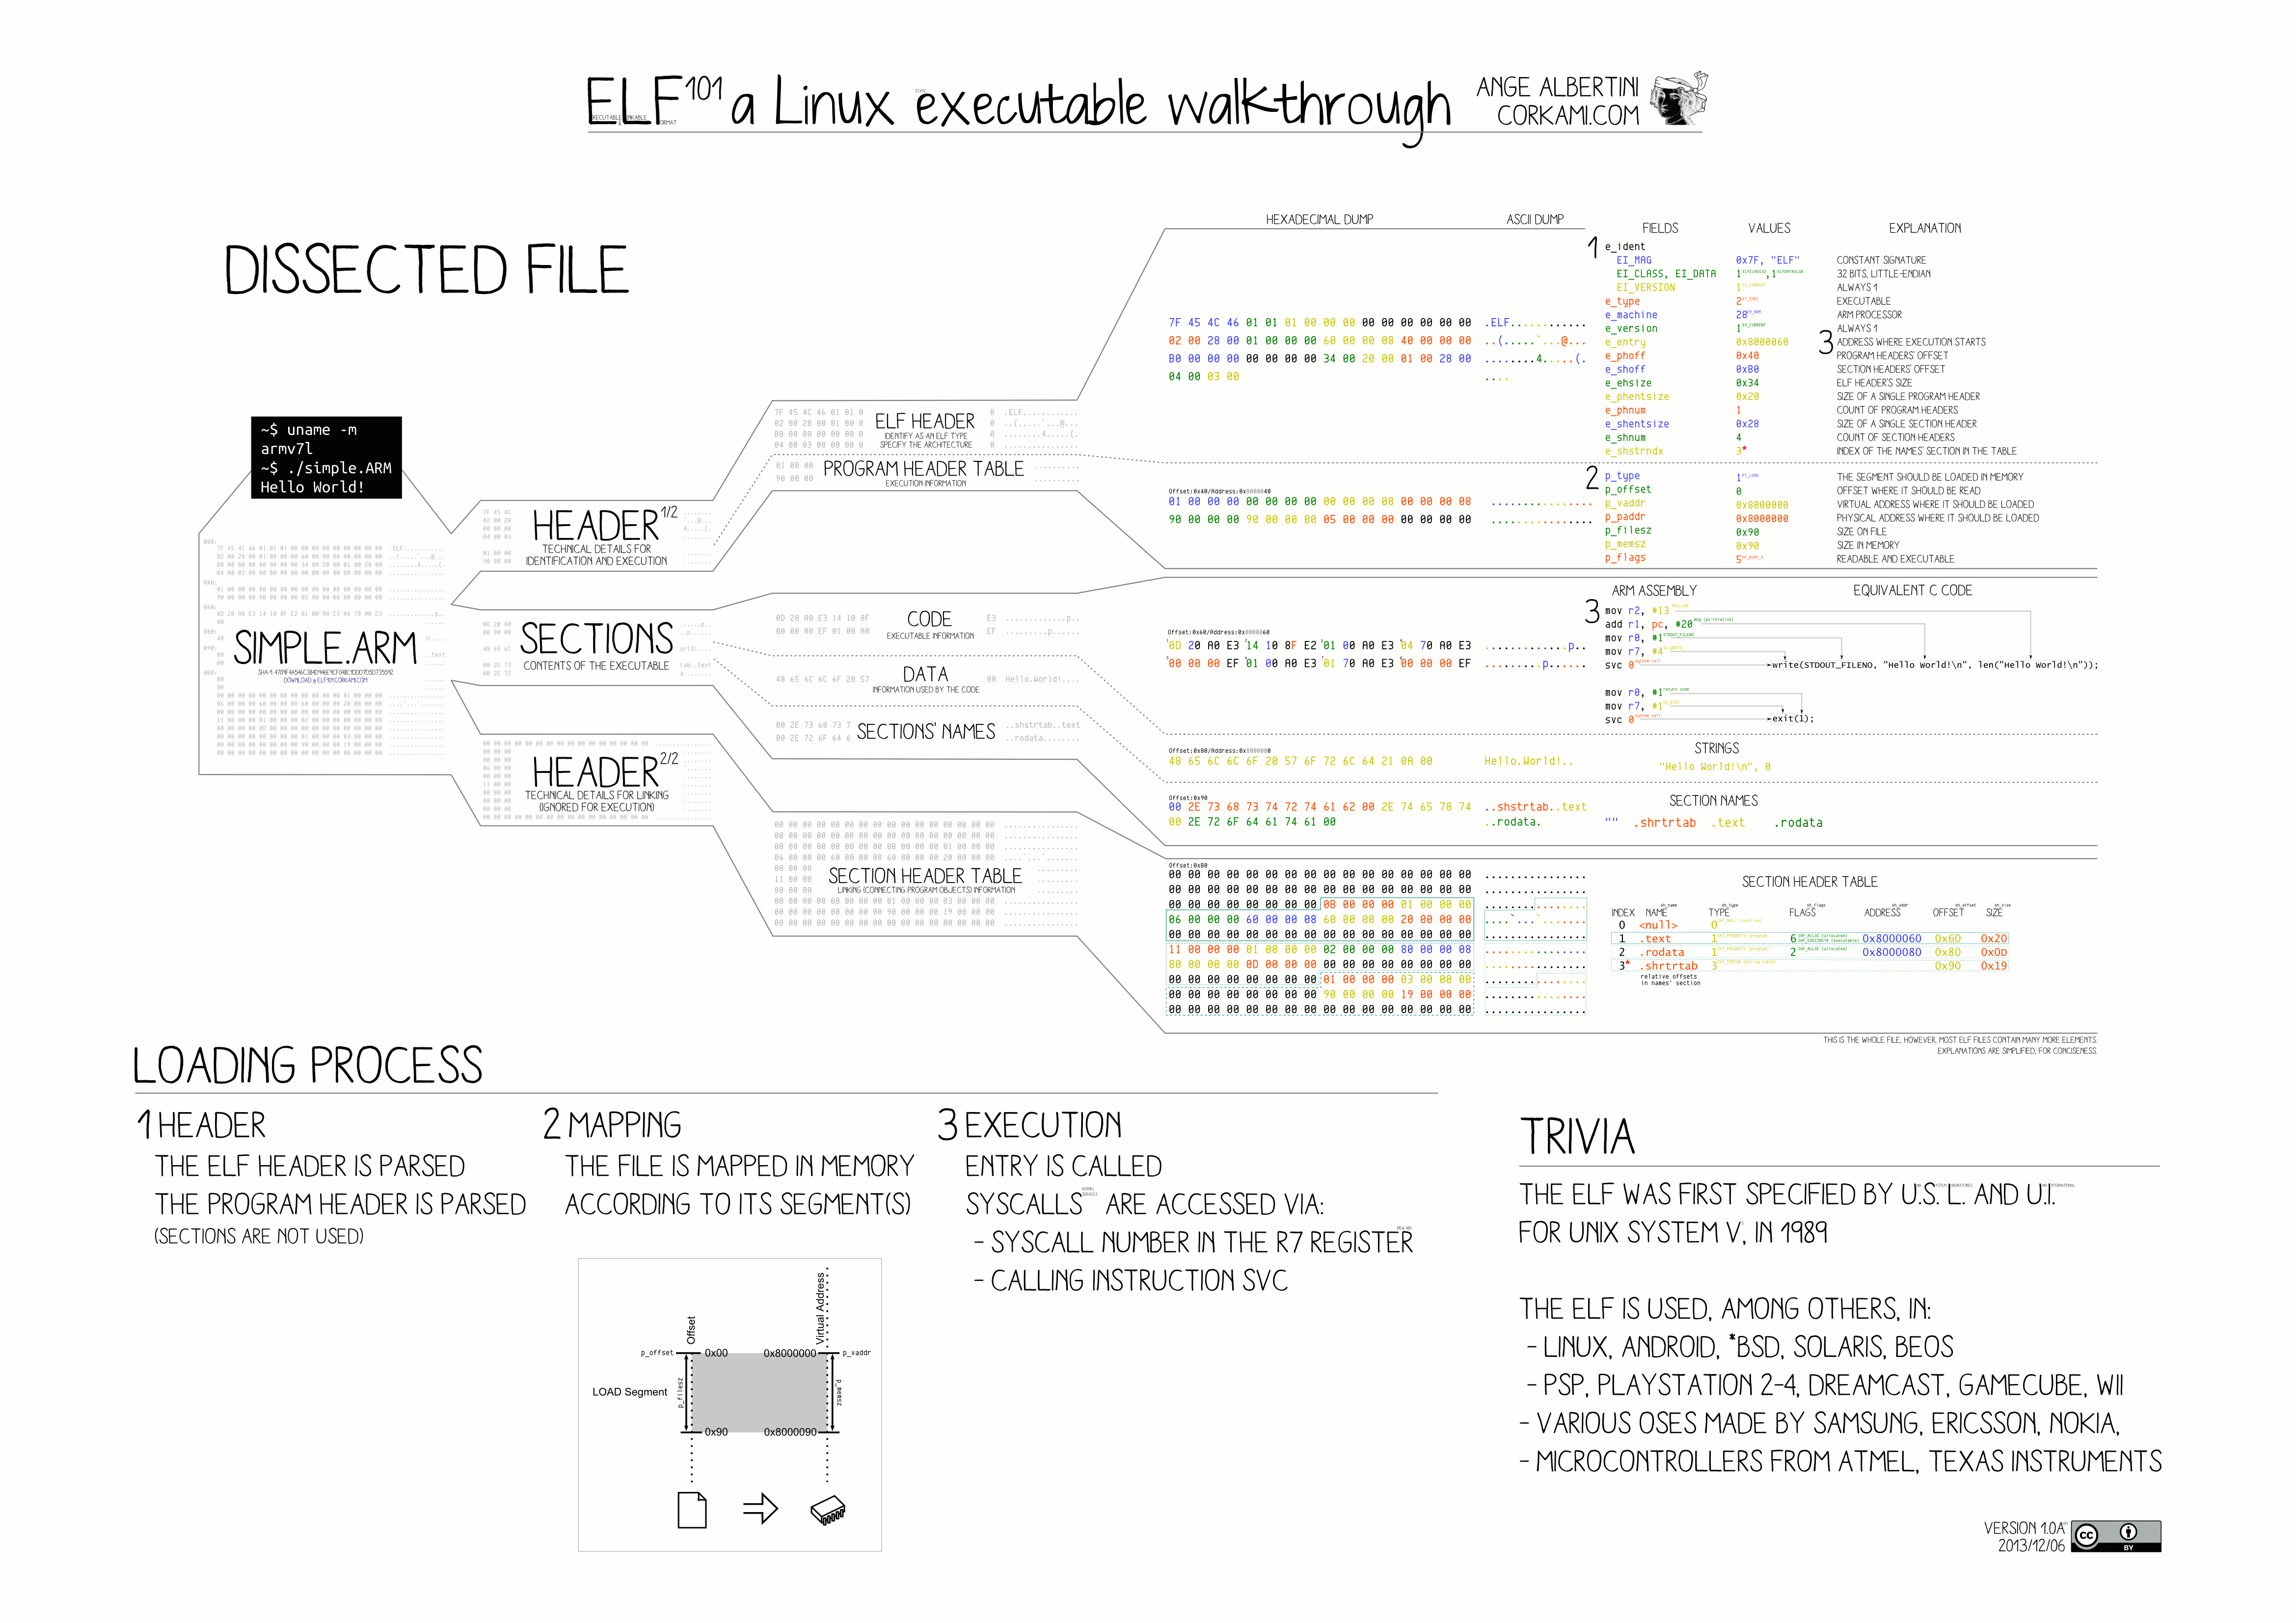
\includegraphics[width=0.5\textwidth]{ELF} \par
}
\quad \par 
代码中还有几点需要注意:(1) 由于映射时需使用 memcpy/memset 函数,
两个函数在地址翻译时使用的是当前 CR3 寄存器所指定的页表,因此需临时
切换至当前进程的页目录,完成映射后再切回内核页目录;(2) 注意到 ELF 镜像
通过一个指针传递,我们可以查看 load\_icode 的调用链,发现其由 env\_create 
负责调用,而 env\_create 调用时使用 env.h 中定义的宏 ENV\_PASTE3,
将调用的位置设置为 \_binary\_obj\_[NAME]\_start,其中 NAME 即为二进制程序的名字。
关于这一系列变量的解释在Lab中也有给出:\underline{这是一种将二进制可执行文件嵌入内核代码的一种方式}。\par
具体地,在 kern/Makeflag 我们可以看到内核链接部分的 flags 中有 \textsl{-b binary} 选项,
这个选项意味着在链接过程中将文件按 raw-format (理论上可以是任意二进制格式)链接而不按 .o 形式解析,
被原封不动嵌入可执行文件中。此外,链接器还会为这些嵌入的二进制文件引入符号注明其位置,即上文
提到的 \_binary\_obj\_[NAME]\_start 的形式:JOS 使用 nm(打印二进制文件中的符号表)命令
将其输出到了 kernel.sym 文件中以便使用者查阅,我们也可以看到这些符号。因此,当内核被加载后,
这些被嵌入的 raw-ELF 也被加载到内存中,并且其位置由上述链接器提供的全局符号标志,故load\_icode
(以及后文出现的env\_create())可以直接使用这些全局符号找到这些嵌入的ELF。

\newpage
\quad \par 
\lstset{style=CStyle}
\setmainfont{Consolas}
\begin{lstlisting}
static void
load_icode(struct Env *e, uint8_t *binary)
{
    // LAB 3: Your code here.
    struct Elf *elf = (struct Elf *)binary;
    if(elf->e_magic != ELF_MAGIC)
        panic("load_icode: e_magic != ELF_MAGIC.\n");

    struct Proghdr *pht = (struct Proghdr *)(binary + elf->e_phoff);

    lcr3(PADDR(e->env_pgdir)); // for valid-use of memcpy/memset
    for(int i = 0; i < elf->e_phnum; ++i)
    {
        if(pht[i].p_type == ELF_PROG_LOAD)
        {
            // Allocate physical regions
            region_alloc(e, (void *)pht[i].p_va, pht[i].p_memsz);
            // Copy the contents from ELF
            memcpy(
                (void *)pht[i].p_va, 
                (void *)(binary) + pht[i].p_offset,
                pht[i].p_filesz
            );
            // Set the rest to be zero
            if(pht[i].p_filesz < pht[i].p_memsz)
                memset(
                    (void *)pht[i].p_va + pht[i].p_filesz,
                    0,
                    pht[i].p_memsz - pht[i].p_filesz
                );
            
        }
    }
    lcr3(PADDR(kern_pgdir));

    // Setup the entry
    e->env_tf.tf_eip = elf->e_entry;	

    // Now map one page for the program's initial stack
    // at virtual address USTACKTOP - PGSIZE.
    // LAB 3: Your code here.
    region_alloc(e, (void *)(USTACKTOP-PGSIZE), PGSIZE);
}
\end{lstlisting}
\setmainfont{Times New Roman}

\newpage
\subsection{\large env\_create \& env\_run}
env\_create 用于创建新进程并载入二进制程序,env\_run 功能则为切换
当前执行的进程。代码实现如下:\par 
\quad \par 
\lstset{style=CStyle}
\setmainfont{Consolas}
\begin{lstlisting}
void
env_create(uint8_t *binary, enum EnvType type)
{
    // LAB 3: Your code here.
    struct Env *new_env = NULL;
    if(env_alloc(&new_env, 0) < 0)
        panic("env_crate: env_alloc failed.\n");
    new_env->env_type = type;
    load_icode(new_env, binary);
}

void
env_run(struct Env *e)
{
	// Step 1: If this is a context switch (a new environment is running):
	//	   1. Set the current environment (if any) back to
	//	      ENV_RUNNABLE if it is ENV_RUNNING (think about
	//	      what other states it can be in),
	//	   2. Set 'curenv' to the new environment,
	//	   3. Set its status to ENV_RUNNING,
	//	   4. Update its 'env_runs' counter,
	//	   5. Use lcr3() to switch to its address space.
	// Step 2: Use env_pop_tf() to restore the environment's
	//	   registers and drop into user mode in the
	//	   environment.
    // ...
	// LAB 3: Your code here.
	if(curenv)
	{
		if(curenv->env_status == ENV_RUNNING)
			curenv->env_status = ENV_RUNNABLE;
	}
	curenv = e;
	curenv->env_status = ENV_RUNNING;
	curenv->env_runs++;
	// !Use physic addr of pgdir
	lcr3(PADDR(curenv->env_pgdir));
	env_pop_tf(&(curenv->env_tf));
}
\end{lstlisting}
\setmainfont{Times New Roman}

\newpage
在上述部分代码完成后,Lab 让我们实现一个调试:首先在 env\_pop\_tf 处设置断点后执行,
通过查阅 kernel 源码我们知道当前内核启动后会创建第一个用户进程 hello 并使用 env\_run 运行它,
env\_pop\_tf 就发生在这次调用中。当 env\_pop\_tf 完成后,执行流进入用户进程的运行状态。此时 
Lab 要求我们在 hello 进程中的 int \$0x30 处打断点并执行,再单步执行后可发现内核发生 fault。\par
\quad \par 
{
\centering
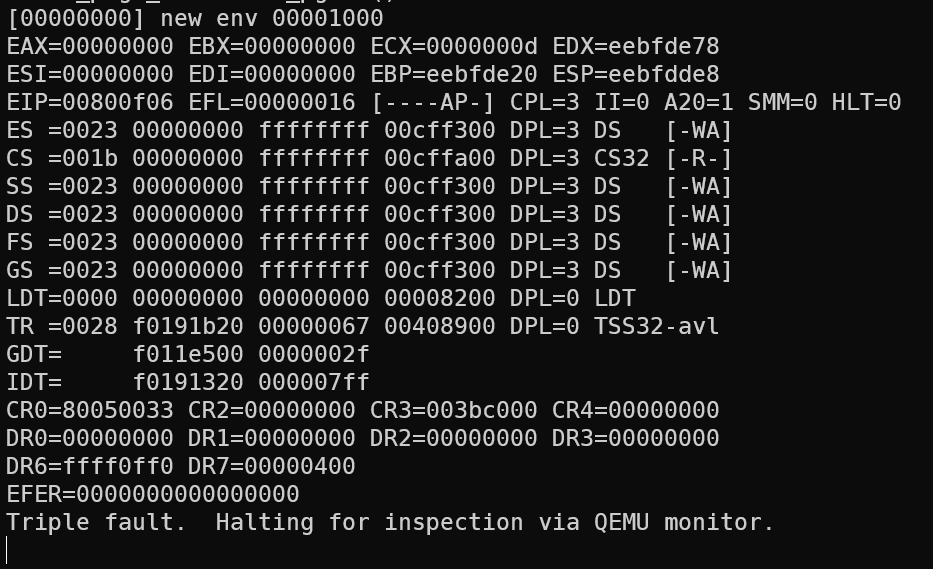
\includegraphics[width=0.7\textwidth]{hellofault} \par
}
\quad \par 
查看 hello.c 与 hello.asm 并结合内核打印的信息我们可以得知该 fault 在打印 "hello world!" 语句时
发生;检查调用链可知,vcprintf 在调用 sys\_cputs() 时产生了一个 syscall,该 syscall 调用出现问题的 
int \$0x30 指令。由此我们基本可以确认,这个 fault 是由于缺少处理 syscall 的中断处理程序而产生的。\par
此处我们还需厘清一个问题是:\underline{JOS是在哪里完成对用户态/内核态的区分的}?也即,我们分配的进程
在哪里被设置为用户态程序? \par
我们知道在 x86 中,一段内容处于 Ring x 记录在当前 CS 寄存器中的 CPL 位,这一位通常与该段内容
所处段的段选择子 DPL 位相等,因此设置一段内容的 Ring x 权限,必然涉及 GDT 的设置。我们使用 IDE 
的搜索功能查询 GDT 相关关键字,很快就能找到相关代码:env\_init\_percpu():\par
\newpage
\lstset{style=CStyle}
\setmainfont{Consolas}
\begin{lstlisting}
// Load GDT and segment descriptors.
void
env_init_percpu(void)
{
    lgdt(&gdt_pd);
    // The kernel never uses GS or FS, so we leave those set to
    // the user data segment.
    asm volatile("movw %%ax,%%gs" : : "a" (GD_UD|3));
    asm volatile("movw %%ax,%%fs" : : "a" (GD_UD|3));
    // The kernel does use ES, DS, and SS.  We'll change between
    // the kernel and user data segments as needed.
    asm volatile("movw %%ax,%%es" : : "a" (GD_KD));
    asm volatile("movw %%ax,%%ds" : : "a" (GD_KD));
    asm volatile("movw %%ax,%%ss" : : "a" (GD_KD));
    // Load the kernel text segment into CS.
    asm volatile("ljmp %0,$1f\n 1:\n" : : "i" (GD_KT));
    // For good measure, clear the local descriptor table (LDT),
    // since we don't use it.
    lldt(0);
}
\end{lstlisting}
\setmainfont{Times New Roman}
这段代码使用 gdt\_pd 变量的内容更新了当前的GDT,同时设置了当前内核代码的CS,ES,
DS,SS寄存器为 GD\_KD 段选择子的位置。我们查看 gdt\_pd 的内容:\par
\lstset{style=CStyle}
\setmainfont{Consolas}
\begin{lstlisting}
struct Segdesc gdt[] =
{
    // 0x0 - unused (always faults -- for trapping NULL far pointers)
    SEG_NULL,
    // 0x8 - kernel code segment
    [GD_KT >> 3] = SEG(STA_X | STA_R, 0x0, 0xffffffff, 0),
    // 0x10 - kernel data segment
    [GD_KD >> 3] = SEG(STA_W, 0x0, 0xffffffff, 0),
    // 0x18 - user code segment
    [GD_UT >> 3] = SEG(STA_X | STA_R, 0x0, 0xffffffff, 3),
    // 0x20 - user data segment
    [GD_UD >> 3] = SEG(STA_W, 0x0, 0xffffffff, 3),
    // 0x28 - tss, initialized in trap_init_percpu()
    [GD_TSS0 >> 3] = SEG_NULL
};

struct Pseudodesc gdt_pd = {
    sizeof(gdt) - 1, (unsigned long) gdt
};
\end{lstlisting}
\setmainfont{Times New Roman}
\newpage 
从上述代码我们就可以看到,新的 GDT 仍然采用 flat-pattern 的方式来忽略分段机制,
但利用了段选择子的权限位设置实现内核态和用户态的权限区分(内核段为Ring0,代码段为
Ring3)。所有用户态进程均有内核分配及初始化,因此内核的权限设置工作应当也由内核代码实现。
同样进行搜索后发现,在分配进程的函数 env\_alloc() 中就进行了相应设置,
由此我们便可以理解操作系统如何提供运行在Ring3的用户态进程了:\par 
\quad \par 
\lstset{style=CStyle}
\setmainfont{Consolas}
\begin{lstlisting}
int
env_alloc(struct Env **newenv_store, envid_t parent_id)
{

...
    // Set up appropriate initial values for the segment registers.
	// GD_UD is the user data segment selector in the GDT, and
	// GD_UT is the user text segment selector (see inc/memlayout.h).
	// The low 2 bits of each segment register contains the
	// Requestor Privilege Level (RPL); 3 means user mode.  When
	// we switch privilege levels, the hardware does various
	// checks involving the RPL and the Descriptor Privilege Level
	// (DPL) stored in the descriptors themselves.
	e->env_tf.tf_ds = GD_UD | 3;
	e->env_tf.tf_es = GD_UD | 3;
	e->env_tf.tf_ss = GD_UD | 3;
	e->env_tf.tf_esp = USTACKTOP;
	e->env_tf.tf_cs = GD_UT | 3;
...

}
\end{lstlisting}
\setmainfont{Times New Roman}


\newpage
\section[\large Handling Interrupts and Exceptions]{Handling Interrupts and Exceptions}

\exercise{3}{
    \par 
    {
        Read \underline{Chapter 9, Exceptions and Interrupts} in the 80386 Programmer's Manual 
        (or Chapter 5 of the \underline{IA-32 Developer's Manual}), 
        if you haven't already.
    } \par
}
\subsection{\large Interrupts \& Exceptions}
通常情况下,\textbf{外部中断(External Interrupts)}可以被分为两类:
中断(Interrupts)和异常(Exceptions)。其中两者可以被进一步细分。

\begin{itemize}
    \item[·]\textbf{中断(Interrupts):}
    分为可屏蔽中断(Maskable Interrupts)与不可屏蔽中断(Nonmaskable Interrupts),
    前者由CPU的INTR引脚发出信号产生,后者由NMI引脚产生。一般来说不可屏蔽中断都由致命错误
    引发,通常的处理方式不是为其设置 Handler,而是直接发出错误警告终止程序。\par 
    \underline{一般认为中断信号是异步信号,由CPU外设备产生}。
    \item[·]\textbf{异常(Exceptions):}
    异常通常分为(1)由CPU自行检测到的异常,会被进一步分类为 trap/fault/abort,例如divide zero异常;
    (2)还有部分信号是可编程的,例如INT 0x3指令触发,也被称为软中断(Software Interrupts)。\par
    与中断相对的,\underline{异常信号通常为同步信号},即由当前CPU运行中的代码产生的。
\end{itemize}

\subsection{\large Enabling and Disabling Interrupts}
中断与异常屏蔽方式有以下几种:
\begin{itemize}
    \item[·]\textbf{NMI Masks Further NMIs:}\par 
    当一个NMI处理程序进行中时,其他的NMI会被暂时屏蔽,直到处理程序执行结束。
    \item[·]\textbf{IF Masks INTR:} \par 
    通过设置IF(interrupt-enable flag)可以开启/关闭可屏蔽中断。x86提供 CLI/STI 指令
    设置该位(bootloader.S中使用过该指令)。
    \item[·]\textbf{RF Masks Debug Faults:} \par 
    设置EFLAGS中的RF位可以开启/关闭 debug fault。
    \item[·]\textbf{MOV or POP to SS Masks Some Interrupts and Exceptions:} \par 
    这是一类应对不正常行为的中断屏蔽。如果在修改SS寄存器与ESP寄存器之间产生了中断,
    会产生SS:ESP的不一致性,可能影响中断处理程序的行为。因此,在修改SS寄存器时(MOV/POP)
    80386架构会禁止NMI、INTR及异常中断,仅有page fault与general protection fault会发生。
    \underline{改为使用LSS指令可以避开这个问题处理}。
\end{itemize}

\newpage
\section[\large Basics of Protected Control Transfer]{Basics of Protected Control Transfer}
为实现从用户态到内核态切换的同时保证对用户态可执行内容的限制,
x86提供了两种机制:{\bf 中断向量表(Interrupt Descriptor Table, IDT)}及
{\bf 任务状态段(Task State Segment, TSS)}。\par 
\subsection{\large Interrupt Description Table (IDT)}
IDT的形式与GDT类似,地址存储在专门的寄存器 IDTR 中。IDT提供一个256 entries的表记录
处理不同类型中断/异常的函数入口,当异常发生时调用对应的函数(加载handler的EIP/CS)。
IDT中包含三种不同的表项,如下图所示:\par 
{
\centering
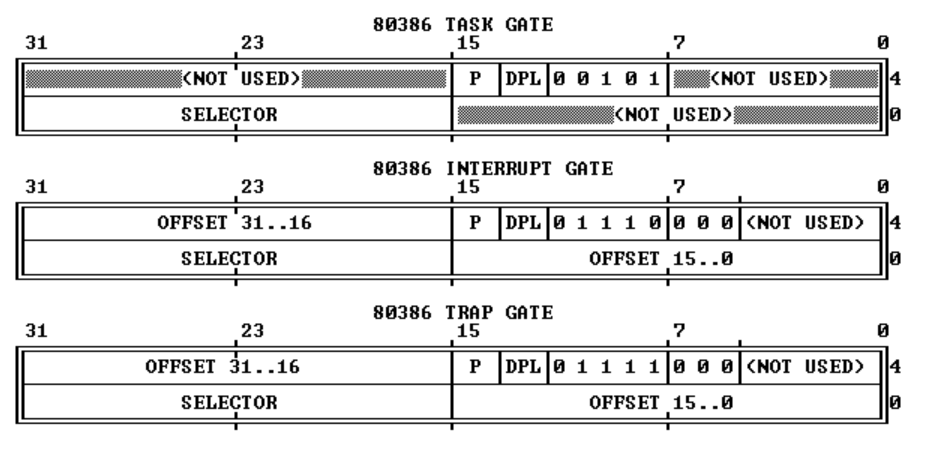
\includegraphics[width=0.7\textwidth]{IDTD} \par
}
\quad \par 

\subsection{\large Task State Segment (TSS)}
当调用中断处理程序时,需要我们保存当前执行流的现场以便完成异常处理后恢复执行。
而且应当注意的是,执行流现场必须保存到高特权级的位置,否则可能遭到其他用户态带
bug或恶意的代码的影响。\par 
当发生中断/异常且handler向更高特权级转换时,x86会切换当前使用的栈到高特权级栈
(内核栈)。同时,x86定义了 TSS 作为保存现场的数据结构,发生异常时将记录执行流相关信息
的TSS压入内核栈中。\par 
TSS结构保存着大量信息,JOS仅使用 ESP0 及 SS0 两个域,用于指定切换的内核栈位置。
\underline{TSS的地址被保存在TR寄存器中,可以通过LTR/STR指令进行操作}。JOS在trap\_init\_percpu()
中执行了TSS段的初始化加载。

\newpage
\section[\large Types of Exceptions and Interrupts]{Types of Exceptions and Interrupts}
在x86中,所有的(同步)异常被分配到 0-31 号中断向量上,即IDT的前32个entries,例如 page-fault 就使用
14号中断向量。\par
大于31号的中断向量被用于处理软件中断,可能的来源是int指令发送的中断及外部设备中断等异步中断。
在Lab3中,我们会实现JOS对0-31号所有同步异常处理入口的设置以及系统调用中断的设置(JOS使用了
中断号0x30,这个选择是可任意的);在Lab4中会进一步拓展至可以处理时钟中断等外部中断。
x86中发射中断向量的指令是\underline{int n 指令},它完成以下任务:\par
\begin{itemize}
    \item[·]根据索引n在IDT中找到处理函数的入口; \par
    \item[·]检查CS寄存器的权限位(CPL); \par
    \item[·]将当前ESP寄存器及SS寄存器存放入CPU内部空闲寄存器; \par
    \item[·]从TSS中加载\underline{内核栈}的ESP寄存器及SS寄存器; \par
    \item[·]将原有的ESP寄存器、SS寄存器(两者当前暂时存放于CPU其他寄存器中)等入\underline{内核栈}; \par
    \item[·]将EFLAGS寄存器、当前进程的CS寄存器及IP寄存器入(内核栈);\par
    \item[·]将CPU控制交给处理函数(处理函数负责调用 iret 命令从中断处理中返回)。 \par
\end{itemize}
到这里,int 指令已经完成了填充内核栈信息的一部分工作,内核栈内容如下图所示:\par 
\quad \par 
{
\centering
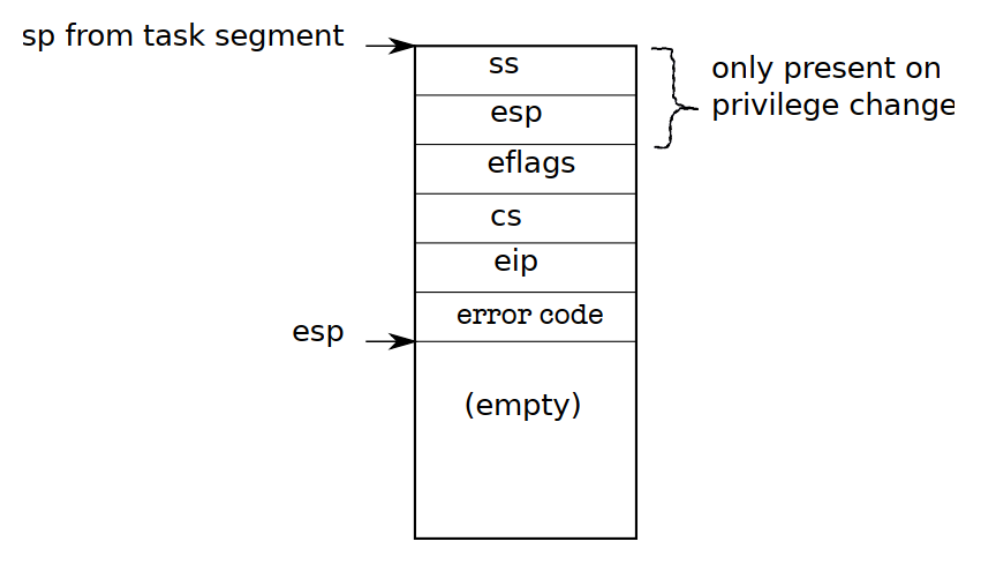
\includegraphics[width=0.7\textwidth]{interrupt_kstack} \par
}

为进一步填充完整信息(形成TrapFrame),trap 入口函数提供进一步操作,如下图所示。
JOS的做法是在每个入口函数将 trapno 入栈后,统一进入 \_alltrap 函数处理(Exercise 4内容)。\par 
\newpage
{
\centering
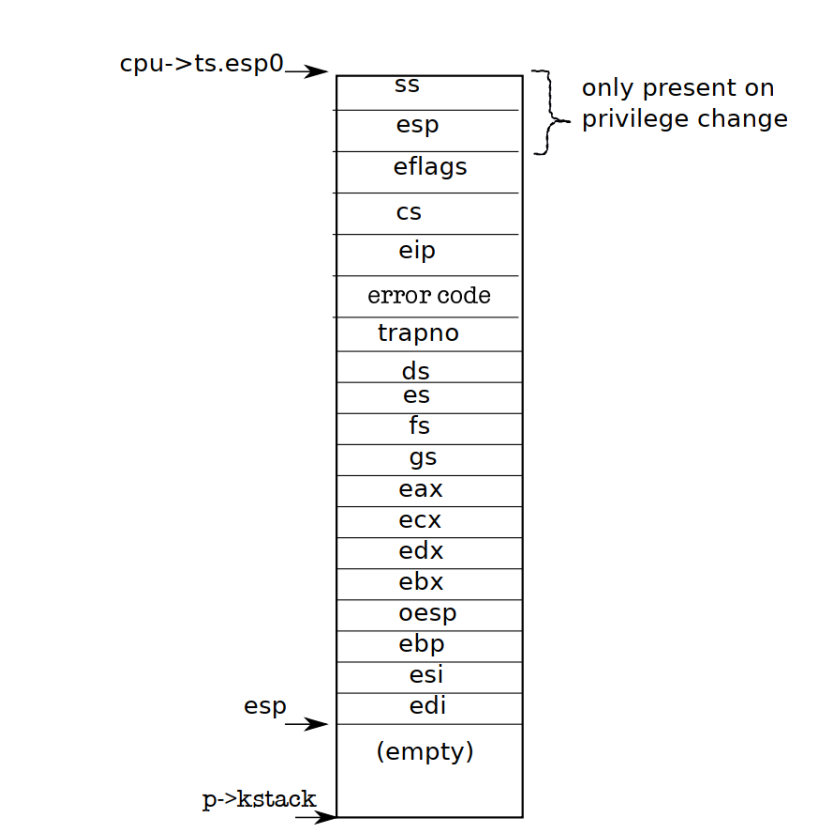
\includegraphics[width=0.7\textwidth]{trap_frame} \par
}



\section[\large Nested Exceptions and Interrupts]{Nested Exceptions and Interrupts}
当已经处于内核态时,也可以继续嵌套处理中断和异常,
此时会在内核栈中继续装填处理帧,唯一不同的是不会再将SS和ESP寄存器入栈。\par


\section[\large Setting Up the IDT]{Setting Up the IDT}
\exercise{4}{
        \par 
        {
            Edit trapentry.S and trap.c and implement the features described above. 
            The macros \underline{TRAPHANDLER} and \underline{TRAPHANDLER\_NOEC} in trapentry.S 
            should help you, as well as the T\_\* defines in inc/trap.h. 
            You will need to add an entry point in trapentry.S 
            (using those macros) for each trap defined in inc/trap.h, 
            and you'll have to provide \_alltraps which 
            the TRAPHANDLER macros refer to. 
            You will also need to modify trap\_init() to initialize 
            the idt to point to each of these entry points 
            defined in trapentry.S; 
            the \underline{SETGATE} macro will be helpful here.
        } \par
        {
            Test your trap handling code using 
            some of the test programs in the user directory 
            that cause exceptions before making any system calls, 
            such as user/divzero. 
            You should be able to get make grade to succeed 
            on the divzero, softint, and badsegment tests 
            at this point.
        } \par
}
\quad \par 

Part A最后一部分要求修改 trapentry.S 及 trap.c 文件,对IDT进行初始化。 
trapentry.S 提供了两个宏: TRAPHANDLER与TRAPHANDLER\_NOEC 用于生成处理函数入口
(与xv6中的 vectors.pl 功能相近)。设置代码如下: 
\lstset{style=AssemblyStyle}
\setmainfont{Consolas}
\begin{lstlisting}
/*
* Lab 3: Your code here for generating entry points for the different traps.
*/
TRAPHANDLER_NOEC(DIVIDE, T_DIVIDE)
TRAPHANDLER_NOEC(DEBUG, T_DEBUG)
TRAPHANDLER_NOEC(NMI, T_NMI)
TRAPHANDLER_NOEC(BRKPT, T_BRKPT)
TRAPHANDLER_NOEC(OFLOW, T_OFLOW)
TRAPHANDLER_NOEC(BOUND, T_BOUND)
TRAPHANDLER_NOEC(ILLOP, T_ILLOP)
TRAPHANDLER_NOEC(DEVICE, T_DEVICE)
TRAPHANDLER(DBLFLT, T_DBLFLT)
TRAPHANDLER(TSS, T_TSS)
TRAPHANDLER(SEGNP, T_SEGNP)
TRAPHANDLER(STACK, T_STACK)
TRAPHANDLER(GPFLT, T_GPFLT)
TRAPHANDLER(PGFLT, T_PGFLT)
TRAPHANDLER_NOEC(FPERR, T_FPERR)
TRAPHANDLER(ALIGN, T_ALIGN)
TRAPHANDLER_NOEC(MCHK, T_MCHK)
TRAPHANDLER_NOEC(SIMDERR, T_SIMDERR)
TRAPHANDLER_NOEC(SYSCALL, T_SYSCALL)
TRAPHANDLER_NOEC(DEFAULT, T_DEFAULT)
\end{lstlisting}
\setmainfont{Times New Roman}
观察两个宏的定义,发现设置后的入口均会跳转至 \_\_alltraps 入口进行通用处理。
这是所有处理函数的通用入口,它填充内核栈使其具有完整的 Trapframe 结构,并根据
Lab提示加载DS、ES寄存器,并将ESP寄存器入栈。
参考xv6源码,对 \_alltraps 补充如下。需要注意的是,JOS 与
x86的 tf 结构略有不同,需进行一定修改;使用了 pushal 指令,即
push all general registers :\par
\lstset{style=AssemblyStyle}
\setmainfont{Consolas}
\begin{lstlisting}
 .global _alltraps
_alltraps:
	pushl %ds
	pushl %es
	pushal
	movw $GD_KD, %ax
	movw %ax, %ds
	movw %ax, %es
	pushl %esp
	call trap
\end{lstlisting}
\setmainfont{Times New Roman}

\newpage
观察可知,这段代码最终跳转至 trap.c/trap() ,由该函数进行分发与中断处理。
参考xv6,我们需要正确设置trap的入口使其可以跳转至handler,
也即设置IDT。这一步骤在 trap.c/trap\_init() 函数中完成:
\lstset{style=CStyle}
\setmainfont{Consolas}
\begin{lstlisting}
void
trap_init(void)
{
    extern struct Segdesc gdt[];

    // LAB 3: Your code here.
    extern void DIVIDE();
    extern void DEBUG();
    ...
    extern void SYSCALL();
    extern void DEFAULT();

    SETGATE(idt[T_DIVIDE], 0, GD_KT, DIVIDE, 0);
    SETGATE(idt[T_DEBUG], 0, GD_KT, DEBUG, 0);
    SETGATE(idt[T_NMI], 0, GD_KT, NMI, 0);
    SETGATE(idt[T_BRKPT], 0, GD_KT, BRKPT, 3); // !
    SETGATE(idt[T_OFLOW], 0, GD_KT, OFLOW, 0);
    SETGATE(idt[T_BOUND], 0, GD_KT, BOUND, 0);
    SETGATE(idt[T_ILLOP], 0, GD_KT, ILLOP, 0);
    SETGATE(idt[T_DEVICE], 0, GD_KT, DEVICE, 0);
    SETGATE(idt[T_DBLFLT], 0, GD_KT, DBLFLT, 0);
    SETGATE(idt[T_TSS], 0, GD_KT, TSS, 0);
    SETGATE(idt[T_SEGNP], 0, GD_KT, SEGNP, 0);
    SETGATE(idt[T_STACK], 0, GD_KT, STACK, 0);
    SETGATE(idt[T_GPFLT], 0, GD_KT, GPFLT, 0);
    SETGATE(idt[T_PGFLT], 0, GD_KT, PGFLT, 0);
    SETGATE(idt[T_FPERR], 0, GD_KT, FPERR, 0);
    SETGATE(idt[T_ALIGN], 0, GD_KT, ALIGN, 0);
    SETGATE(idt[T_MCHK], 0, GD_KT, MCHK, 0);
    SETGATE(idt[T_SIMDERR], 0, GD_KT, SIMDERR, 0);
    SETGATE(idt[T_SYSCALL], 1, GD_KT, SYSCALL, 3); // !
    SETGATE(idt[T_DEFAULT], 0, GD_KT, DEFAULT, 0);
    // Per-CPU setup 
    trap_init_percpu();
}
\end{lstlisting}
\setmainfont{Times New Roman}

\newpage 
\question{1}{
    \par 
    \noindent {
        \textsl{Answer the following questions}:
    } \par 
    {
        1. What is the purpose of having an individual handler function 
        for each exception/interrupt? 
        (i.e., if all exceptions/interrupts were delivered to the same handler, 
        what feature that exists in the current implementation 
        could not be provided?)
    }\par 
    {
        2. Did you have to do anything to make the user/softint program behave correctly? 
        The grade script expects it to produce a general protection 
        fault (trap 13), but softint's code says int \$14. 
        Why should this produce interrupt vector 13? 
        What happens if the kernel actually allows softint's int \$14 
        instruction to invoke the kernel's page fault handler 
        (which is interrupt vector 14)?
    }\par 
}
\quad \par 
尝试回答上述问题。\par 
1. 不同的中断对应不同的问题,应当采取不同的处理方式,很难进行统一化处理。\par 
2. user/softint 程序原本应该产生 13 号中断(尽管其int指令发射的是14号中断),
因为该程序运行在Ring 3权限级,而根据 IDT 的定义我们知道14号中断需要DPL=0,因此
在用户态发射14号中断将引发越权异常,从而触发13号中断。如果内核允许用户态代码使用14号
Page Fault 中断,可能导致有bug的或者恶意程序耗竭系统的内存资源导致崩溃。\par 

% ---- Part B ---------------------------------
\chapter[\Large Page Faults, Breakpoints Exceptions, and System Calls]{Page Faults, Breakpoints Exceptions, and System Calls}

\section[\large Handling Page Faults]{Handling Page Faults}

\exercise{5}{
    \par 
    {
        Modify trap\_dispatch() to dispatch page fault exceptions to page\_fault\_handler(). 
        You should now be able to get make grade to succeed on the faultread, faultreadkernel, 
        faultwrite, and faultwritekernel tests. 
        If any of them don't work, figure out why and fix them. 
        Remember that you can boot JOS into a particular user program using 
        \textsl{make run-x} or \textsl{make run-x-nox}. 
        For instance, \textsl{make run-hello-nox} runs the hello user program.
    } \par
}
这一节练习的内容较为简单,要求我们将 PageFault 异常分配给它对应的处理函数。我们仅需修改
trap\_dispatch 函数即可:\par 

\lstset{style=CStyle}
\setmainfont{Consolas}
\begin{lstlisting}
static void
trap_dispatch(struct Trapframe *tf)
{
    // Handle processor exceptions.
    // LAB 3: Your code here.
    switch(tf->tf_trapno)
    {
        case T_PGFLT:
            page_fault_handler(tf);
            break;
    }
    ...
}
\end{lstlisting}
\setmainfont{Times New Roman}

\newpage
\section[\large The Breakpoint Exception]{The Breakpoint Exception}

\exercise{6}{
    \par 
    {
        Modify trap\_dispatch() to make breakpoint exceptions invoke the kernel monitor. 
        You should now be able to get make grade to succeed on the breakpoint test.
    } \par
}
这一步实验也十分简单,我们在上一个 Exercise 的代码基础上追加即可:\par

\lstset{style=CStyle}
\setmainfont{Consolas}
\begin{lstlisting}
static void
trap_dispatch(struct Trapframe *tf)
{
    // Handle processor exceptions.
    // LAB 3: Your code here.
    switch(tf->tf_trapno)
    {
        case T_PGFLT:
            page_fault_handler(tf);
            break;
        case T_BRKPT:
            monitor(tf);
            break;
    }
    ...
}
\end{lstlisting}
\setmainfont{Times New Roman}

\challenge{1}{
    \par 
    {
        Modify the JOS kernel monitor so that you can 'continue' execution from the current location 
        (e.g., after the int3, if the kernel monitor was invoked via the breakpoint exception), 
        and so that you can single-step one instruction at a time. 
        You will need to understand certain bits of the EFLAGS register in order to 
        implement single-stepping.
    }\par 
}
\quad \par 

【待完成】

\newpage
\question{2}{
    \par 
    {
        3. The break point test case will either generate a break point exception or 
        a general protection fault depending on how you initialized the break point entry 
        in the IDT (i.e., your call to SETGATE from trap\_init). Why? 
        How do you need to set it up in order to get the breakpoint exception 
        to work as specified above and what incorrect setup would cause it 
        to trigger a general protection fault?
    }\par 
    {
        4. What do you think is the point of these mechanisms, 
        particularly in light of what the user/softint test program does?
    }\par 
}
\quad \par 
尝试回答上述问题。\par 
3. 在 SETGATE 阶段如果将 DPL-bit 设置为3则触发breakpoint,否则(DPL=0)则触发 general protection fault。
这是因为 breakpoint 用户程序处在Ring 3权限级,若设置DPL!=3将导致其无权限发送 int \$3 指令,从而触发地址保护异常。\par 
4. 上述所有的机制都是为用户态代码提供“有限”访问权限的保障。\par 

\end{document}